\documentclass{article}
\pdfpagewidth=8.5in
\pdfpageheight=11in
\usepackage{ijcai18}
% The file ijcai18.sty is the style file for IJCAI-18 (same as ijcai08.sty).

% Use the postscript times font!
\usepackage{times}
\usepackage{soul}
\usepackage{url}
\usepackage[hidelinks]{hyperref}

\usepackage[utf8]{inputenc}
\usepackage[english]{babel}
\usepackage[small]{caption}

%%%%%%
\newtheorem{theorem}{Theorem}

% Math notation
\RequirePackage[group-separator={,}]{siunitx}
\newcommand{\na}{$\mathrm{N.A.}$}
\newcommand{\minus}{\scalebox{0.7}[1.0]{$-$}}
\newcommand{\expn}[1]{\!\!\times\!\!10^{\minus#1}}
\newcommand{\pval}[2]{$p\textrm{-value} = #1\expn{#2}$}
\newcommand{\set}[1]{\{{}#1\}}
\newcommand{\A}[1]{\mathcal{A}_{#1}}
\newcommand{\N}[1]{n_{#1}(j)}



%%%%%%
\usepackage{float}
\usepackage{listings}
\usepackage{caption}
\usepackage{graphicx}
\usepackage{subcaption}
\usepackage{colortbl}
\usepackage{amsmath}
%\usepackage{amsthm} 
\usepackage{mathpartir}
\usepackage{fancyvrb}\fvset{fontsize=\small}
\usepackage{xspace}
\usepackage{xcolor}
\usepackage{balance}
\usepackage{wrapfig}
\usepackage{multirow}
\usepackage{pifont}
\usepackage{amssymb}
%%%%%%%%%%%%%%%%%%% this can reduce space quite a lot
\usepackage{soul}
\usepackage{microtype}
\usepackage[T1]{fontenc}
\usepackage{dsfont}
%%%%%%%%%%%%%%%%%%% this can reduce space quite a lot
\usepackage{relsize}
\usepackage{tikz}
\usepackage{longtable}
\usepackage{booktabs}
\usepackage{marvosym} 
\usepackage{framed}
\usepackage{mdwlist}
\usepackage{tabularx}
\usepackage{wrapfig}

\usepackage{array}
\usepackage{mathtools}
\usepackage{url}
\usepackage{color}

%% Colors
\definecolor{bgBlock}{rgb}{0.22,0.15,0.49}
\definecolor{bgBlockAlert}{rgb}{0.99,0.84,0.31}
\definecolor{fgBlockAlert}{rgb}{0.22,0.15,0.49}
\definecolor{fgBlock}{rgb}{0.99,0.84,0.31}
\definecolor{darkred}{rgb}{0.5,0,0}
\definecolor{darkgreen}{rgb}{0,0.5,0}
\definecolor{darkblue}{rgb}{0,0,0.5}
\definecolor{Gray}{gray}{0.9}

%%%%%%%%%% added by sofia
\usepackage{algpseudocode}
\usepackage{algorithm}
\usepackage{enumitem}


\usepackage{bm}
\usepackage{cleveref}
\usepackage{textcomp}
\usepackage{pdfpages}
\usepackage{chngpage}


%\usepackage[hyphenbreaks]{breakurl}


%%%%%%%%%%

\usepackage[most]{tcolorbox}
\newtcolorbox{myframe}[1][]{
	enhanced,
	arc=0pt,
	outer arc=0pt,
	colback=white,
	boxrule=0.5pt,
	boxsep=1pt,left=3pt,right=3pt,top=5pt,bottom=5pt,
	fontupper=\small,
	size=small
	#1
}

%%%%%%%%%%
% appendix 
\usepackage[toc,page]{appendix}
\usepackage{makecell}


%%%%% Theorem -> Claim

\newtheorem{thm}{Theorem} % the main one
\newtheorem{lemma}[thm]{Lemma}

\newcommand{\thistheoremname}{}
\newtheorem{genericthm}[thm]{\thistheoremname}
\newenvironment{namedthm}[1]
  {\renewcommand{\thistheoremname}{#1}
   \begin{genericthm}}
  {\end{genericthm}}





\newcommand{\Fix}[1]{\textbf{[[}{\color{red} #1}\textbf{]]}}
\newcommand{\Anonim}[2]{#1}
\newcommand{\ie}{i.e.}
\newcommand{\eg}{e.g.}
\newcommand{\cf}{cf.}
\newcommand{\etal}{et al.}
\newcommand{\comments}[1]{}
\newcommand{\varex}{\textsc{Varex}}
\newcommand{\tsig}{OUR}
\newcommand{\tnamepar}[1]{\tname{}\texttt{[#1]}}
\newcommand{\CodeIn}[1]{{\small\texttt{#1}}}
\newcommand{\pw}{\textsc{pw}}
\newcommand{\pwopt}{\textsc{pw-opt}}
\newcommand{\dd}{\CodeIn{DD}}
\newcommand{\acrAbrev}{APR}
\newcommand{\RQ}{RQ}
\newcommand{\morpho}{\emph{morpho}}
\newcommand{\lithium}{\emph{lithium-slicer}}
\newcommand{\success}{\leavevmode\color[HTML]{009901}}

\definecolor{bs}{rgb}{0.59, 0.0, 0.09}
\definecolor{d}{HTML}{800000}

\newcommand{\BS}[1]{\textbf{[BS:[}{\color{bs} #1}\textbf{]]}}
\newcommand{\Mar}[1]{\textbf{[Marcelo:[}{\color{orange} #1}\textbf{]]}}
\newcommand{\Sof}[1]{\textbf{[Sofia:[}{\color{cyan} #1}\textbf{]]}}
\newcommand{\oururl}{\Fix{url here}}
\newcommand{\tname}{\Fix{Critical Slicing Revisited}}

\newcommand{\numPrograms}{six}
\newcommand{\numFaults}{395}
\newcommand{\topk}{top-$k$}

\newcommand{\sfl}{SFL}
\newcommand{\CS}{CS}
\newcommand{\cs}{CS}
\newcommand{\ds}{DS}
\newcommand{\dfj}{Defects4J}
\newcommand{\orbs}{ORBS}
\newcommand{\comb}{\sfl{}+\ds{}}
\newcommand{\apr}{APR}

%% subject names as in https://github.com/rjust/defects4j
\newcommand{\chart}{JFreechart}
\newcommand{\closure}{Closure compiler}
\newcommand{\lang}{Apache commons-lang}
\newcommand{\cmath}{Apache commons-math}
\newcommand{\mockito}{Mockito}
\newcommand{\jtime}{Joda-Time}

\newcommand{\cmark}{\ding{51}}%
\newcommand{\xmark}{\ding{55}}%


% the following package is optional:
\usepackage{latexsym}

\title{Demystifying the Dynamic Slicing and SFL Combination}

% \author{
% First Author$^1$,
% Second Author$^2$,
% \\
% $^1$ First Affiliation\\
% $^2$ Second Affiliation\\
% %
% first@email.address,
% second@email.address,
% third@email.address
% }

% If your authors do not fit in the default space, you can increase it
% by uncommenting the following (adjust the "2.5in" size to make it fit
% properly)
% \setlength\titlebox{2.5in}

\hypersetup{draft}
\begin{document}

\maketitle

\begin{abstract}
  Software debugging is important and challenging. This paper reports
  on a comprehensive study to reassess the impact of combining two
  very popular automated techniques for software fault
  localization--Dynamic Slicing and Spectrum-based Fault
  Localization. Our results show that \Fix{...}
\end{abstract}

\section{Introduction}

Software debugging is difficult. In particular, the task of locating the faulty
code (\ie{}, fault localization) is particularly challenging. For that reason,
countless automated techniques have been proposed in the past to reduce the cost
of fault localization~\cite{7390282}.

%% Although the technique has been intensively investigated in
%% research, few use cases gained notoriety---WhyLine~\cite{Ko:2008:DRA:1368088.1368130} being an
%% exception.


Model-based software diagnosis (MBSD)~\cite{REITER198757,DEKLEER200325} and Spectrum-Based Fault Localization
(\sfl{}) are two very popular techniques that leverage different principles
to automate fault isolation. An example of a MBSD is Dynamic
Slicing~\cite{Agrawal:1990:DPS:93542.93576}
as wel as some work~\cite{Perez:2018:LQR:3304889.3304927}\Rui{Cite Wolgang Mayer, ASE2008, IJCAI, DX, ... as well as
some works of Wotawa}, a technique that traces back statements
in the code that influence some point of interest, such as the evaluation
of a failing assertion. In contrast to \ds{}, \sfl{}~\cite{7390282}
does not analyze code. Instead, it is a black-box, statistical fault
localization method that computes suspiciousness values associated
with program entities (e.g., methods) based on coverage information gathered
during the execution of test cases as well as the
output of test cases. More precisely, \sfl{} uses coverage information
of passing and failing test cases to identify likely faulty
statements and produces on output a list of program entities ranked in
decreasing order of suspiciousness.
\ds{} and \sfl{} are complementary debugging techniques~\cite{DBLP:conf/sac/AbreuGZG08}.
Intuitively, \ds{} identifies irrelevant parts of the code whereas \sfl{}
ranks the relevant parts of the code.

%% Similarly to \ds{}, \sfl{} received
%% tremendous attention in research over the years,
%% but its applicability to support
%% debugging remains
%% questionable~\cite{ang-perez-van-deursen-rui-2017,Pearson:2017:EIF:3097368.3097441,Xie:2016:RAD:2884781.2884834}.
%% Despite the skepticism of the research community, \sfl{} has been
%% shown useful in supporting downstream analyses, such as Automated
%% Program Repair
%% (\apr{})~\cite{automatic-software-repair-survey2017,kim-etal-daghstul2017},
%% an increasingly popular technique that looks for fixes to buggy
%% statements. Tools like JAFF \cite{arcuri-2011}, Prophet
%% \cite{long-rinard-2016}, SemFix \cite{nguyen-qi-roychoudhury-2013},
%% and SPR \cite{long-rinard-2015} use \sfl{} to guide the search for
%% likely fixes.

%% We found surprising that, despite these findings, no tool or client analyses use this combination
%% today.\Sof{@todo: Revise this and look to the paper from 2018} Several reasons could justify that observation. One hypothesis is that results reported in prior work are
%% over-optimistic. For example, most prior work evaluated improvements
%% of \sfl{} techniques using relative metrics, which are based on the
%% position of the first faulty statements found in the ranking relative
%% to the total number of ranked statements, which is often a large
%% number. As such, it inflates actual improvements and deceives
%% potential adopters of the technology. Ang \etal~\cite{ang-perez-van-deursen-rui-2017} recently
%% pointed to that fact and encouraged researchers to adopt more precise metrics,
%% such as \topk{}
%% \cite{Wu:2014:CLC:2610384.2610386,Lucia:2014:FFL:2642937.2642983,Wen:2016:LLB:2970276.2970359},
%% which has been widely adopted to evaluate performance of information retrieval algorithms~\Fix{cite}. This
%% metric reports the percentage of faults captured by a technique when
%% the rank is trimmed to the first $k$ components.

This paper reports the results of a comprehensive study evaluating the
impact of combining \ds{} and \sfl{} to improve software fault
localization, a technique we coin as \comb{}. The intuition for the combination is that
several highly ranked statements, albeit covered by failing
executions, may be unrelated to the fault. Our empirical study involves
\numFaults{} faults from \numPrograms{} different programs comprised
in the Defects4J (D4J) dataset~\cite{just-defects4j-issta2014}, which
is frequently used to evaluate fault localization research. Prior work
reported promising results in this
combination~\cite{Wotawa:2010:FLB:1848650.1849235,Alves:2011:FUD:2190078.2190115,DBLP:conf/ecai/HoferW12,lei-mao-dai-wang-2012,slicing-sfl-repair},
but they used a non-representative set of subjects in their evaluation
or used archaic methods to evaluate technique
improvement~\cite{Wu:2014:CLC:2610384.2610386,Lucia:2014:FFL:2642937.2642983,Wen:2016:LLB:2970276.2970359}.

The goal of this paper is to reassess whether the \comb{} approach
yields promising results under a more rigorous experimental
methodology and a larger dataset.\comments{The D4J dataset is about
  twice as large than the biggest test suite used in previous
  studies.} This study covers the following research questions:

\newcommand{\rqone}{How often does DS miss faulty statements?}
\newcommand{\rqthree}{How effective is the \comb{} approach?}

\begin{itemize}[leftmargin=*]
\item[]{\footnotesize[(un)soundness]}~\textit{\rqone{}}
\item[]{\footnotesize[effectiveness]}~\textit{\rqthree{}}
\end{itemize}

The first question addresses the important problem of missing faulty
statements. Naturally, the consequence of that problem for debugging
is that developers would never be able to locate faults. Different
slicers can miss faulty statements for different reasons. In this
paper, we used Critical Slicing~\cite{DeMillo:1996:CSS:229000.226310},
which, in principle, could miss statements because of imprecise
oracles that guide the slicing process. We evaluated how often that
issue manifests in our experiments. The second research questions
effectively evaluates the impact of the combination. To sum, our
results show that \Sof{@todo: sum up the results}.

The contributions of this work are as follows \Sof{Finish this}:
\begin{itemize}
	\item A comprehensive study on the combination of \sfl{} and \ds{}
     for bug localization of \emph{Java} faulty programs.
   \item A tool that implements \comb{}.
	%\item Empirical evidence that the \comb{} combination improves
\end{itemize}

\section{Background}
\label{sec:background}

This section discusses  important background material for the rest of the paper.
\Rui{not very happy with this sentence.}

\subsection{Critical Slicing (\cs{})}
\label{sec:slicing}

\Rui{intro needs to refer to Critical Slicing, somehow..}
\Rui{Are we the first to use Critical Slicing in combination? Say so, if this
is the case.}
Program slicing is a program understanding technique to identify the
relevant parts of the program with respect to given points of
interest.  Dynamic
slicing~\cite{Agrawal:1990:DPS:93542.93576}\comments{~--~as opposed to
  static
  slicing~\cite{Weiser:1981:PS:800078.802557}~--~~\cite{Binkley:2014:OLP:2635868.2635893}}
has been shown useful in automated software debugging where the region
of interest is restricted to what can be reached from failing
tests. Several dynamic slicing techniques exist. This paper uses
Critical Slicing (\cs{})~\cite{DeMillo:1996:CSS:229000.226310} for its
simplicity/generality.\comments{ In constrast with alternative slicing
  implementations based on dependency
  chains~\cite{Tip:1994:SPS:869354}\comments{(\eg{},
    JSlice~\cite{Wang:2004:UCB:998675.999455} and
    JavaSlicer~\cite{hammacher-bachthesis-2008})},} Critical Slicing
prescribes a black-box language-semantics-agnostic recipe to computing
executable slices.  Critical Slicing simplifies the original
program such that the resulting program preserves critical
observations, such as assertion violations. More precisely, the
simplification mechanism consists of deleting statements on the
original program and checking if the output of the original and
modified program are the same.

Our implementation of Critical Slicing is based on the Mozilla Lithium
tool\footnote{Lithium details available at \url{https://github.com/MozillaSecurity/lithium} (Accessed on \today)}. Lithium implements the DD-min Delta Debugging
algorithm~\cite{zeller-hildebrandt-tse2002}. It takes as input a file
and produces as output a simplified version of that file that
satisfies a user-defined oracle. In our case, the oracle is defined
such that the test produces the same failure manifestation as the one
observed with the test execution on the original program. The
Lithium minimization process starts by determining the initial size---in number of lines---of
chunks to delete from the input file. For that,
it chooses the highest power of two number smaller than the file
size. For example, if the file has 1,000 lines, Lithium sets the
initial chunk size to 512 lines. Then, the tool starts a local search looking
for chunks to exclude from the file. If the chunk satisfies the oracle it is removed.
When no more chunks of that given size can be removed, Lithium
divides the chunk size by two and repeats the search. This iterative
process continues until no more lines can be removed.  If $n$ is the
size of the input file and $m$ is the size of the 1-minimal file found
by Lithium, then Lithium usually performs $O(m\cdot\lg(n))$
iterations. Proofs of the algorithm complexity can be found
elsewhere\footnote{Lithium complexity available at \url{https://github.com/MozillaSecurity/lithium/blob/master/src/lithium/docs/algorithm.md} (Accessed on \today)}. Our implementation is publicly
available at \Rui{site}.

\subsection{Spectrum-based Fault Localization (\sfl)}
\label{sec:sfl}

Spectrum-based fault localization is a statistical fault
localization technique that takes as input a test suite including at
least one failing test and reports on output a ranked list of
components likely to be in
fault~\cite{FLSurvey2016,DBLP:conf/kbse/JonesH05,DBLP:journals/smr/LuciaLJTB14,DBLP:journals/jss/AbreuZGG09}. The
following are given in \sfl{}: a finite set $\mathcal{C}=\set{c_1,c_2,...,c_M}$ of $M$ system \emph{components}\footnote{A
  component can be any code artifact of arbitrary granularity
  such as a class, a method, or a statement~\cite{DBLP:journals/stvr/HarroldRSWY00}.}; a finite set
$\mathcal{T} = \set{t_1,t_2,...,t_N}$ of $N$ system transactions,
which correspond to records of a system execution, such as test cases;
the error vector $e = \set{e_1,e_2,...,e_N}$, where $e_i = 1$ if
transaction $t_i$ has failed and $e_i = 0$ otherwise; and an
$N\times{}M$ coverage matrix $\mathcal{A}$, where $\A{ij}$ denotes the
coverage of component $c_j$ in transaction $t_i$.  The pair
$(\mathcal{A},e)$ is commonly referred to as
spectrum~\cite{DBLP:journals/stvr/HarroldRSWY00}. Figure~\ref{fig:spectrum-example}
shows an example spectrum.
\begin{wrapfigure}[8]{2}{0.3\textwidth}
  \hspace{-2ex}
  \centering
  \scriptsize
  \begin{tabular}{c|cccc|c}
    $\mathcal{T}$ & $c_1$    & $c_2$    & $\cdots$ & $c_M$    & $e$    \\ \hline
    $t_1$         & $\A{11}$ & $\A{12}$ & $\cdots$ & $\A{1M}$ & $e_1$  \\
    $t_2$         & $\A{21}$ & $\A{22}$ & $\cdots$ & $\A{2M}$ & $e_2$  \\
    \vdots        & \vdots   & \vdots   & $\ddots$ & \vdots   & \vdots \\
    $t_N$         & $\A{N1}$ & $\A{N2}$ & $\cdots$ & $\A{NM}$ & $e_N$  \\
  \end{tabular}
  \caption{An example spectrum.}
  \label{fig:spectrum-example}
\end{wrapfigure}

Several types of spectra exist.  The most commonly used is called
hit-spectrum, where the coverage matrix is encoded in terms of binary
\emph{hit} (1) and \emph{not hit} (0) flags, \ie{}, $\A{ij} = 1$ if
$t_i$ covers $c_j$ and $\A{ij} = 0$ otherwise.  \sfl{} takes as input
the pair $(\mathcal{A},e)$ and produces on output a list of components
ranked by their faulty suspiciousness. To that end, the first step of
the technique consists of determining what columns of the matrix $A$
resemble the error vector $e$ the most.  For that, an intermediate
component frequency aggregator $n_{pq}(j)$ is computed $n_{pq}(j) =
|\{i\mid \A{ij}=p \wedge e_i=q\}|$. $n_{pq}(j)$ denotes the number of
runs in which the component $j$ has been active during execution ($p =
1$) or not ($p=0$), and in which the runs failed ($q = 1$) or passed
($q = 0$).  For instance, $n_{11}(j)$ counts the number of times
component $j$ has been involved ($p = 1$) in failing executions ($q =
1$), whereas $n_{10}(j)$ counts the number of times component $j$ has
been involved in passing executions. We then calculate similarity to
the error vector by means of applying \emph{fault predictors} to each
component to produce a score quantifying how likely it is to be
faulty.  Components are then ranked according to such likelihood
scores and reported to the user. Ochiai is one of those fault
predictors that has shown to perform
well~\cite{7390282,Pearson:2017:EIF:3097368.3097441}. The Ochiai
formula is given by the following equation
$\textit{ochiai}\,$=$\,\N{11}/\sqrt{(\N{11}+\N{01}) * (\N{11}+\N{10})}$.
%The Ochiai formula is given by~\cite{DBLP:conf/prdc/AbreuZG06}
%\[ochiai = \frac\]

\section{The \comb{} Approach}
\label{sec:approach}

This section provides details on our \sfl{}+\ds{} combination approach
and its heuristics.

%% \Mar{Sofia, o pseudocodigo acima assume que ha apenas um teste
%%   falho. Isto precisa ser ajustado. O lithium-slicer funciona por caso
%%   de teste ou por suite?  Por favor, ajuste a descricao acima.  Eh um
%%   loop aninhado ao loop ``for every k'' que o lithium-slicer
%%   implementa (algo como ``for every k and every failing test'')?  Caso
%%   vc. faca slice contra um teste particular, vc. garante (checa saida)
%%   que os demais testes que originalmente falhavam continuam falhando
%%   pelo mesmo motivo? Enfim, isto eh bem basico e precisa ficar claro
%%   de inicio.}

%% \Sof{O lithium-slicer funciona por caso de teste. Cada execução da nossa
%% ferramenta chama o lithium tantas vezes como o número de casos de teste
%% que falham para cada versão do projecto. Assumindo que o numero de casos de
%% testes a falhar são 5, numa execução da nossa plataforma o lithium é executado
%% 5x para os 5 testes diferentes. No fim, pega no resultado do slicing de cada
%% teste e actualiza a matrix spectra para calcular o ranking. Eu confiro depois de
%% executar a nossa ferramenta para uma versão do projecto que os
%% testes que aparecem na pasta da versão do projecto são os mesmos quando corro
%% o test do defects4j de novo. Uma precaução que tivemos foi ter a certeza que o
%% oracle que estava a ser usado não sofria com a mudança de máquinas. Portanto,
%% antes de correr as experiências eu corri o defects4j para obter as mensagens
%% esperadas de novo para serem usadas como o oracle esperado. Estas são as verificações
%% que faço. Posso tentar substituir as classes minimizadas nos projectos e ver se
%% realmente a mensagem de erro continua a ser a mesma - coisa que não fiz. Relativamente,
%% ao pseudocode eu diria que é for every $k$ and every failing test.}

\subsection{The \sfl{}+\cs{} combination}
\label{sec:comb}

To illustrate the idea behind the combination of \sfl{} with \cs{}, consider a
debugging scenario with five components $c_{1..5}$ and five
transactions $t_{1..5}$, two of which are failing. Consider,
additionally, that the component $c_2$ is faulty.
Figure~\ref{fig:illustration} shows, at the left-hand side of the
arrow ($\Rightarrow$), an hypothetical spectra and its corresponding
ranking, produced with the Ochiai predictor. Each line in the ranking
shows, respectively, the rank/position, the component label, and the
Ochiai score (in parentheses).

\begin{figure}[t!]

  \centering
  \begin{subfigure}{0.5\textwidth}
    {\def\arraystretch{0.9}\setlength{\tabcolsep}{3pt}
      \begin{tabular}{c|ccccc|c}
        $\mathcal{T}$ & $c_1$    & $c_2$   & $c_3$ & $c_4$ &  $c_5$   & $e$    \\ \hline
        $t_1$         & 1 & 0 & 1 & 1 & 0 &\cmark  \\
        $t_2$         & 0 & 1 & 1 & 1 & 1 &\xmark  \\
        $t_3$         & 1 & 0 & 1 & 0 & 0 &\xmark  \\
        $t_4$         & 0 & 1 & 0 & 0 & 1 &\cmark  \\
        $t_5$         & 1 & 0 & 0 & 1 & 1 &\cmark \\
        \hline
      \end{tabular}
      \quad
      $\Rightarrow$
      \quad
      \begin{tabular}{c|ccccc|c}
        $\mathcal{T}$ & $c_1$    & $c_2$   & $c_3$ & $c_4$ &  $c_5$   & $e$    \\ \hline
        $t_1$         & 1 & 0 & 1 & 1 & 0 &\cmark  \\
        $t_2$         & 0 & 1 & {\cellcolor{Gray} 0} & {\cellcolor{Gray} 0} & 1 &\xmark  \\
        $t_3$         & 1 & 0 & 1 & 0 & 0 &\xmark  \\
        $t_4$         & 0 & 1 & 0 & 0 & 1 &\cmark  \\
        $t_5$         & 1 & 0 & 0 & 1 & 1 &\cmark  \\
        \hline
      \end{tabular}
    }
    \caption{Spectra update.}
    \label{fig:ds-reduction}
  \end{subfigure}

  \vspace{2ex}

  \begin{subfigure}{0.5\textwidth}
    \centering
    \begin{tabular}{cccccc}
      1 & $c_4$ (0.59) & & 1 & $c_2$ (0.35) \\
      2 & $c_3$ (0.55) & & 2.5 & $c_1$ (0.32)\\
      3 & $c_2$ (0.35) & \hspace{1ex}$\Rightarrow$\hspace{1ex} & 2.5 & $c_5$ (0.32)\\
      4.5 & $c_1$ (0.32) & & 4 & $c_3$ (0.29)\\
      4.5 & $c_5$ (0.32) & & 5 & $c_4$ (0.00)\\
    \end{tabular}
    \caption{Ranking update.}
  \end{subfigure}

  \caption{Modifications on spectra and ranking as result of slicing
    code against test $t_2$. Double arrow ($\Rightarrow$) indicates
    before and after.}
  \label{fig:illustration}
  \vspace{-2ex}
\end{figure}

In the following, we illustrate the workflow of the \sfl{}+\cs{}
combination for this scenario. First, the combined technique picks
components $c_4$ and $c_3$, which appear at the top of the ranking,
for further analysis. (The cutoff point is user-defined.) Second, the
technique picks a failing test $t_2$ to slice the code.  Let us assume
that the slice obtained for the transaction $t_2$ is $\{c_2, c_5\}$,
\ie, it excludes components $c_4$ and $c_3$. Finally, the spectra and
ranking are updated. The right-side of Figure~\ref{fig:illustration}
shows the modified spectra and ranking after slicing test $t_2$
against $c_4$ and $c_3$. It is worth noting that the technique slices
the code for every failing tests. More precisely, the workflow of the
\comb{} approach consists of four steps: \Sof{Should we
  specify that these steps are performed for each version of the
  projects/defect?}\Mar{Isn't this clear from the scenario in the
  beginning of par?  Note that this is the definition of the workflow
  for the technique, not the definition of the experiment (when it
  makes sense to talk about versions/defects and D4J.)}\Rui{agree with Marcelo.}
  \Rui{if space permits, a figure with the workflow might be good.}

\begin{enumerate}
  \itemsep0em
  \item\label{step:spectra} Compute spectra $S$ and ranking $R$ for
  the input test suite;
  \item\label{step:susp-files} Select top $k$ most suspicious source
  files\Rui{classes?}, according to $R$;
  \item\label{step:compute-slice} Compute slicer for every suspicious
    file, obtained in Step~\ref{step:susp-files}, and every failing test;
    \Rui{union of slices of all points ?}
  \item Adjust the spectra $S$, obtained in Step~\ref{step:spectra}, with
    the slices obtained in Step~\ref{step:compute-slice} and recompute ranking.
\end{enumerate}

Intuitively, slicing enables identification of cells\Rui{cells?} in the spectra
whose values can be set to zero, \ie{}, the components marked with $0$
are irrelevant to determine the test output. Let us now observe the
effect of this spectra modification on the ranking. Analyzing the
Ochiai formula, one observes that, for the components $j$ which are
not part of the slice of a failing test, the combination reduces the
value of $\N{11}$ and increases the value of $\N{01}$ \Rui{lower case N?}. Therefore,
suspiciousness of those components decrease. Similar argument applies
to other fault predictors. In the running example,
Figure~\ref{fig:illustration}, components $c_3$ and $c_4$, which are
not in the slice of $t_2$, have their suspiciousness reduced, enabling
the faulty component $c_2$ to rise from the third to the first
position in the ranking.

\begin{theorem}
  The faulty statement may not be included in the critical slice of
  failing test cases.
\end{theorem}

Conceptually, if the oracles implemented in faulty tests are too
general, the critical slicing algorithm could produce slices without
the faulty code. For example, consider the scenario of an unexpected
Null-Pointer Exception (NPE) thrown in the code. If the oracle checks
for the presence of NPE regardless of where it occurs, it is possible,
in principle, that the final slice does not include the faulty code
but still raises NPE (in a different part of the code). The critical
slicing algorithm would consider that as an acceptable simplification
and would continue. Section~\ref{sec:oracleheuristics} shows how we
mitigate this fundamental limitation of Critical Slicing and
Section~\ref{sec:fault-misses} shows how problematic is that issue in
practice.

%% \vspace{3mm}
%% \begin{myframe} \label{box:1}
%% \textbf{java.lang.NullPointerException}, \\
%% at org.jfree.data.general.junit.DatasetUtilitiesTests.\\
%% testBug2849731$\_$3(DatasetUtilitiesTests.java:1299), \\
%% ...
%% \end{myframe}

\begin{theorem}
  The rank of faulty statements cannot decrease if the slice includes
  the faulty statements.
\end{theorem}

The proof is based on the outlined argument that irrelevant
components $j$ have their ranks reduced as $\N{11}$ decreases and
$\N{01}$ increases. If those irrelevant components appear at positions
above the faulty component, it is possible that the faulty component
becomes more suspicious relative to $j$, \ie{}, the ranking of the
faulty component increases. If those components appear at positions
below the faulty components, the ranking of the faulty components is
unaffected.


\subsection{Oracle Heuristics}
\label{sec:oracleheuristics}

% \subsection{Implementation}
% \label{sec:impl}

% \Mar{Sofia, I think this was way too low-level for intro and decided
%   to move here. please check how to fit.}
% \Fix{
% A couple of different tools were designed to perform this empirical study: \morpho{} and \lithium{}. \morpho{} retrieves as an output the input for \lithium{}. \lithium{} uses the input to reduce the search domain for \sfl{} and outputs the statements that resulted from the minimization. \morpho{} uses this to update the spectrum matrix, performs the before and after \sfl{} evaluation using the corresponding matrix, and outputs the metrics that report the \sfl{} performance for both cases ~---~ before and after using \ds{}. }

% Two different tools were developed to support this research: \morpho{} and \lithium{}. \morpho{} was designed to calculate the suspiciousness of all statements of a project before, and after the top-k minimization performed by \lithium{} whereas \lithium{} is responsible for reducing the search domain of each \texttt{Java} class of the project for the after-\sfl{} analysis. \morpho{} uses the spectrum matrix (Figure \ref{fig:spectrum-example}), and the pair \emph{name\#location} for each statement to calculate the respective ranking. All rankings are ordered from highest to lowest ranked. This information is retrieved along with each test case stack trace in a \texttt{.json} file which serves as an output to \lithium{}. \lithium{} starts by generating the inputs (Algorithm \ref{alg:ls}, line $2$) for the top-k classes of each failing test based, mainly, on the output of \emph{morpho} ~---~ ranked list of statements and the test cases stacktraces. Then, the tool iterates each class from the top-k classes ($c$) of each test $t$. In each iteration, classes are refined using an external java program (Algorithm \ref{alg:ls}, line 6) that substitutes all the line comments ($\backslash\backslash$), block comments ($\backslash*$ to $*\backslash$) and javadoc comments ($/**$ to $*/$) using the \texttt{JavaParser}\footnote{JavaParser is available at http://javaparser.org/ (accessed November 2018).} library. This step was added to \lithium{} because it turns \texttt{MozillaLithium} faster since the empty lines are ignored. Then, \texttt{MozillaLithium} performs the class minimization using a function of interest (Algorithm \ref{alg:finc}) which compares the output of the test with the expected one which is given as an input. Finally, the location of all relevant statements (Algorithm \ref{alg:ls}, line 9) is saved in a \texttt{.json} which is used for the before-\sfl{} analysis. \morpho{} uses the output from \lithium{} to create a copy of the older spectrum matrix and updates it according to the explanation provided on Figure \ref{fig:ds-reduction} where the statements that are not in the slice of the test suffer a suspiciouness reduction. In the end, \morpho{} performs the \sfl{} analysis for both matrixes and calculates the probability of the first line being faulty, the probability of the last line being faulty, and the mean and median of the position of the faulty line in the ranking. These are the metrics used to evaluate how considerable is the improvement obtained when combining \ds{} with \sfl{}.

% \begin{algorithm}[h]
% 	\caption{Class Minimization Algorithm}
% 	\label{alg:ls}
% 	\begin{flushleft}
% 		\textbf{Input:} $proj$ - project name \\
% 		\hspace{2.75em} $bug$ - bug number\\
% 		\hspace{2.75em} $k$ - number of top ranked classes\\
% 		\hspace{2.75em} $stk$ - expected stacktrace\\
% 	 \textbf{Output:} Top-k classes minimization for each test \\
% 	\end{flushleft}
% 	\begin{algorithmic}[1]
% 		\Procedure{lithium-slicer}{$proj$, $bug$, $k$, $stk$}
% 			\State $testsInfo \leftarrow$ generateInputs($proj$, $bug$, $k$, $stk$)
% 			\ForAll {$t \in testsInfo$}
% 				\State $classes \leftarrow$ getClasses($proj$, $bug$)
% 				\ForAll {$c \in classes$}
% 					\State $unc \leftarrow$ removeComments($c$)
% 					\State $min \leftarrow$ MozillaLithium($iFunc$, $unc$, $t$, $stk$)
% 				\EndFor
% 				\State $slicer \leftarrow$ getLocation($c$, $t$, $min$)
% 			\EndFor
% 			\State \Return $slicer$
% 		\EndProcedure
% 	\end{algorithmic}
%
% \end{algorithm}
%
% \begin{figure*}[t]
% 	\centering
% 	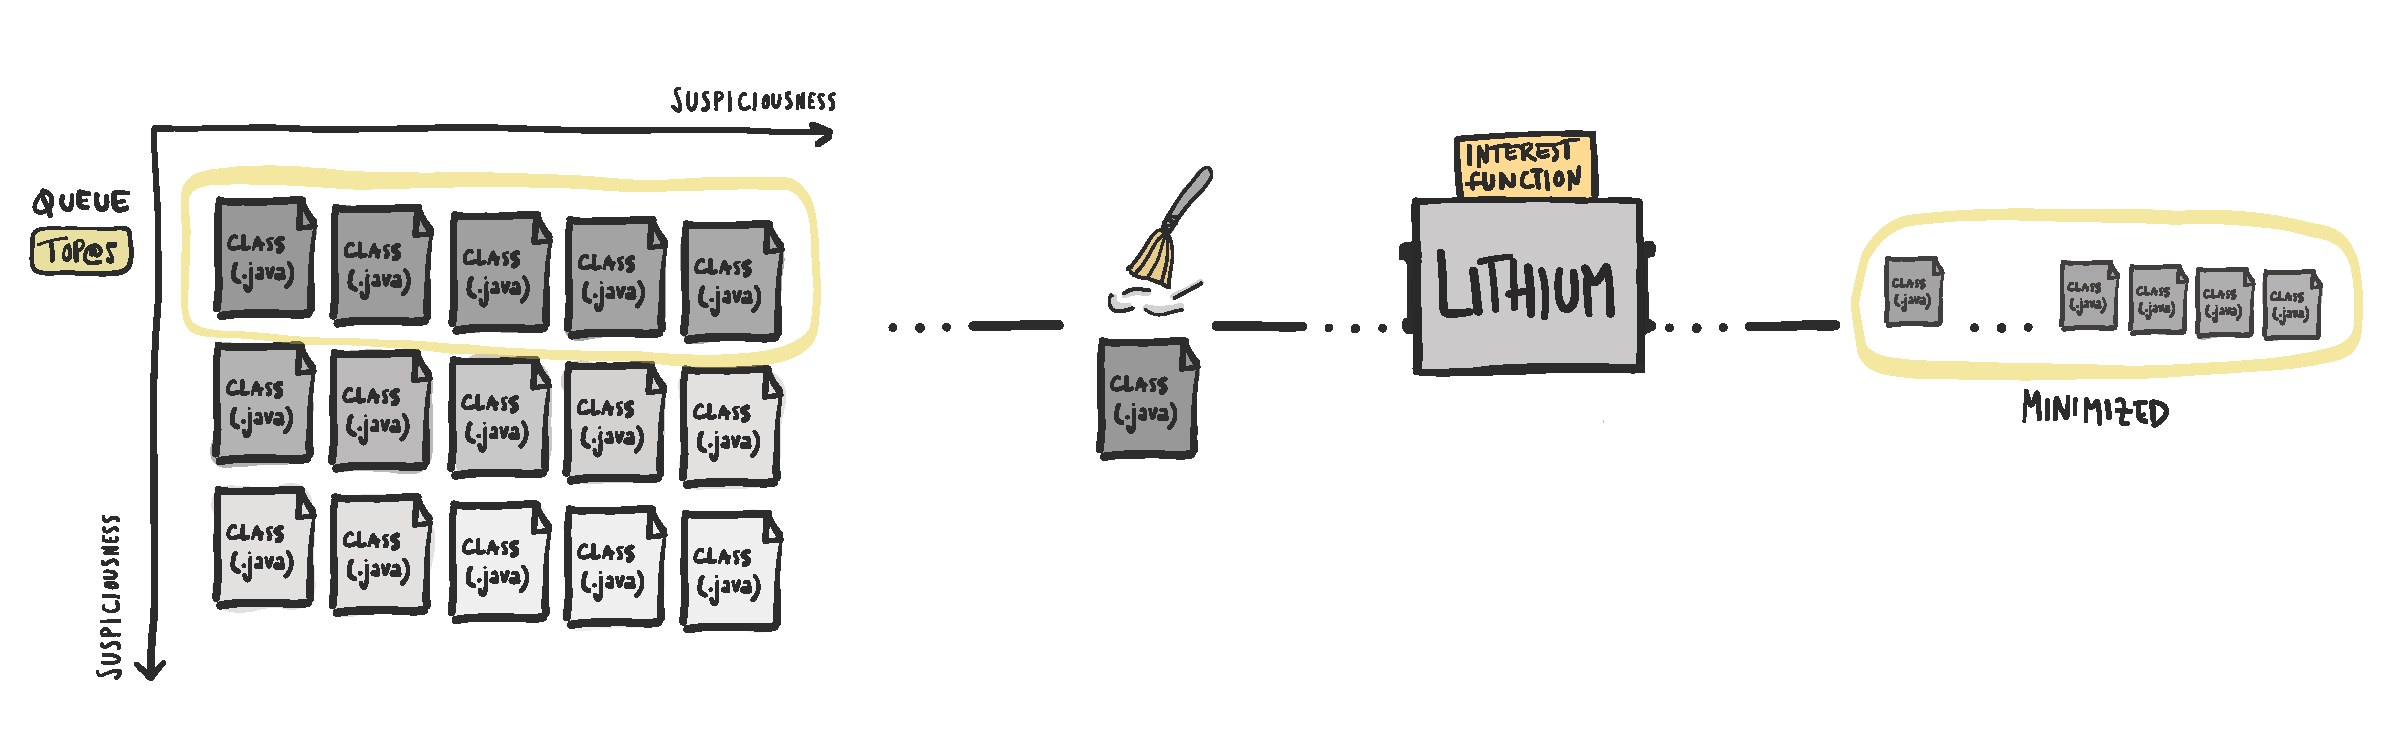
\includegraphics[width=1.0\textwidth]{figures/lithium.pdf}
% 	\caption{Simple illustration of the process to obtain the top-5 minimized classes from a project carrying a bug}
% \end{figure*}
%
% \subsection{Function of Interest }
% \label{sec:funcofint}
%
%

\Mar{I left a bunch o comments to Sofia on hangouts...$\rightarrow$}
\Rui{This is too rought. I would not talk about lithium right away.}
Lithium takes as input a function of interest that can be designed according to the problem to be solved. The function of interest determines if the test case output is interesting or not. In this study, interesting means that the test execution path is equal to the expected one. This information can be deducted from the defects stack traces which show the stack of functions called until the thrown of an exception. The interesting function compares both stack traces (from the test under evaluation and the expected one) until the call where the test fails. For each chunk under evaluation, the test is executed after the chunk being deleted from the source code . Both test ($testStk$) and expected ($expStk$) stack traces are filtered. We only consider stack traces until the line where the main exception is launched. These operations are performed by line 3 and 4 from Algorithm 2. Finally, both messages are compared and if equal the chunk will be deleted from the project, i.e., the chunk is not interesting to reveal the fault of the test.

% \begin{algorithm}[h]
% 	\caption{Function of interest (iFunc)}
% 	\label{alg:finc}
% 	\begin{flushleft}
% 		\textbf{Input:} $c$ - class to be minimized\\
% 		\hspace{2.75em} $t$ - testcase name\\
% 		\hspace{2.75em} $expStk$ -  expected stacktrace\\
% 		\textbf{Output:} $interest$ - $True$ if it is interesting, $False$ if not \\
% 	\end{flushleft}
% 	\begin{algorithmic}[1]
% 		\Function{iFunc}{$c$, $t$, $expStk$}
% 		\State $testStk \leftarrow$ runTest($t$)
% 		\State $testOracle \leftarrow$ getOracleToCompare($testStk$)
% 		\State $expOracle \leftarrow$ getOracleToCompare($expStk$)
% 		\State \Return $testOracle$ == $expOracle$
% 		\EndFunction
%
% 	\end{algorithmic}
%
% \end{algorithm}

\section{Evaluation}
\label{sec:eval}

To evaluate our approach, we compare the cost of diagnosing
a collection of faulty versions using \sfl{} versus \comb{}.

\subsection{Objects of Analysis}\label{sec:analysis}

We used the \dfj{} benchmark in our
experiments~\cite{just-defects4j-issta2014}. This benchmark includes
six different subjects and \numFaults{} faults (Table \ref{tab:df4j}).
\lang{} is a library that provides a set of helper utilities for the
     {\small\texttt{java.lang}} API. \cmath{} is a lightweight library
     of self-contained mathematics and statistics components. The
     \closure{} is a toolset for turning JavaScript files into smaller
     scripts for faster download and execution in the
     browser. \chart{} is a Java library for creating charts. \jtime{}
     is a lightweight library that aims to replace the default Java
     {\small\texttt{java.util.Date}} classes providing simpler
     APIs. \mockito{} is a mocking testing framework.

\newcommand{\cgray}[1]{\cellcolor{gray!25}#1}
\begin{table}[h]
  \centering
  \setlength{\tabcolsep}{4pt}
    \begin{tabular}{lrrr}
      \toprule
      Project            & Size (LOC) & \# Tests & \# Faults \\ %\comments{& Failing Test Cases &}
      \midrule
      \lang{}            & 111,751  & 6,057 & 65       \\   %\commentst{& 124   &  -}\\
      \cmath{}           & 306,276  & 26,797 & 106     \\   %\comments{& 177   &  -}\\
      \closure{}         & 149,521  & 27,930  & 133     \\   %\comments{& 350   &  -}\\
      \chart{}           & 230,159  & 8,458 & 26      \\  %\comments{& 92    &  -}\\
      \jtime{}           & 141,610  & 3,289 & 27       \\   %\comments{& 76    &  -}\\
      \mockito{}         & 22,787  & 8,835 & 38    \\     %\comments{& 118   &  -}\\
      \bottomrule
  \end{tabular}
\caption {Characterization of \dfj{} subjects.\Sof{Use SLOCCount to count size}}
\label{tab:df4j}
\end{table}
\normalsize

\Sof{@todo: Add pie chart to show the distribution of foos}

\subsection{Experimental Methodology}\label{sec:methodology}

%% The main goal of our evaluation is to understand what is the impact of
%% \ds{} on \sfl{} after minimizing the $k$ highest faulty source files
%% which comprise the highest faulty statements.

Recall from Section~\ref{sec:approach} that the \comb{}
takes as input a value $k$ that denotes the $k$ most suspicious distinct
classes to be considered. To evaluate the effectiveness of \comb{}, following
related work, we compared its
performance with \sfl{} for each defect on each subject program from
the dataset, for $k\in\{5,10\}$. These classes are obtained directly
from the ranking. We refer to these variations as \combpar{k}. We
compared \combpar{5} and \combpar{10} against \sfl{} using the
following metrics.\Mar{Sofia, I don't see a reason for an equation to
  only show the difference of cost. Please describe precisely the
  metrics. In this case, I can't find what C stands for. Also,
 you need to describe precisely what top@n (or someother name) means
 in this context. Check if it makes sense for SFL.$\rightarrow$}\Rui{It might
 be good to keep it just to give it some emphasis... }


\begin{equation}
    \Delta{}C = C(\textrm{SFL}) - C(\textrm{\combpar{k}})
\end{equation}

\noindent
where $C$ is the cost of diagnosis. \Rui{At this point, you need to explain what
the cost of diagnosis is: C is the number of statemetns (?) that need to be
inspected before finding the fault, right? We also need to say that we assume a
perfect bug understanding: that is, when the developer sees the bug in the
ranking, he can say that it is the faulty one.}
A positive $\Delta$C means that the position of the faulty statement has decreased
in the ranking reported computed by \combpar{k}. Hence, reducing the cost to
find the bug.

\subsection{Dynamic Slicing}
\Rui{ehmm.. what is this section all about? }


\begin{table}[h]
	\centering
	\setlength{\tabcolsep}{4pt}
	\begin{tabular}{lcc}
		\toprule
		Project             &  \combpar{k}  & \combpar{10} \\
		\midrule

        \lang{}            & 0.77\% & 30.28\%\\
        \cmath{}           &  & \\
        \closure{}          &  & \\
		\chart{}			& 59.30\% & 53.64\% \\
        \jtime{}            & 17.27\% & 32.92\%\\
        \mockito{}          & 16.99\% & 21.67\%\\

		\bottomrule
	\end{tabular}
	\caption {\ds{} reduction performance for each version of the \chart{} project considering only the top-5 and top-10 classes}
	\label{tab:red}
\end{table}
\normalsize

Table \ref{tab:red} reports the reduction of statements after using \ds{} to minimize the top-5 and top-10 of classes of the subjects.


\subsection{Results}
\Rui{Results \& Discussion?}

The following section aims to answer the research questions presented previously.


\subsubsection{RQ1: \textit{How often DS misses faulty statements?}}
\label{sec:fault-misses}

In \textbf{RQ1}, we evaluate how often \ds{} misses faulty statements, since it is one of the main problems of dynamic slicing techniques.

Table \ref{table:fsws} presents the number of faults where at least one of the faulty statements appears in the final reports of both techniques, \sfl{} and \comb{}-k.


\begin{table*}[h]
	\centering
	  \begin{tabular}{|l|ccc|cccc|c|}
		\toprule
		\multirow{2}{*}{Project}            & \multicolumn{3}{c|}{SFL}  & \multicolumn{4}{c|}{\combpar{k}} & \multirow{2}{*}{\# Faults} \\

		            & \% $k = 5$ & \% $k = 10$  & $\Delta$ & \# $k = 5$ & \% $k = 5$ & \# $k = 10$ & \% $k = 10$ &  \\
		\midrule
		 \lang{}            & 84.1\%  & 84.1\%  &  0\%   & 63 & 100\% & 61 & 96.8\% & 63      \\
		% \cmath{}           & 82.08 \%  & 85.85 \% & 3.77 \%     \\   %\comments{& 177   &  -}\\
		% \closure{}         & 62.41 \%  & 72.18 \%  & 9.77 \%     \\   %\comments{& 350   &  -}\\
		\chart{}           & 84.6\%  & 92.3\% & 7.7\%  & 20 & 76.9\% & 22 & 84.6\% & 26    \\  %\comments{& 92    &  -}\\
		\jtime{}           & 77.8 \%  & 100.0 \% & 22.2 \%  & 22 & 81.5\% & 23 & 85.2\% & 27     \\   %\comments{& 76    &  -}\\
		 \mockito{}         & 63.2\%  & 71.1\% & 7.9\%   & 27 & 71.1\% & 30 & 79.0\% & 38 \\     %\comments{& 118   &  -}\\
		\bottomrule
	\end{tabular}
  \caption {Number of faults where at least one of the buggy-lines is in the SFL and \combpar{k} report \Sof{@todo: Add absolute numbers for SFL}\Rui{explain what $k$ is for SFL alone.}}
  \label{table:fsws}
\end{table*}

% \begin{table*}[h]
% 	\centering
% 	\setlength{\tabcolsep}{4pt}
% 	\begin{tabular}{llllll}
% 		\toprule
% 		Project             &  \# top-5  & \% top-5 & \# top-10 & \% top-10 & \# Faults \\
% 		\midrule
% 		\chart{}  & 20 & 76.92\% & 22 & 84.62\%  & 26\\
% 		\jtime{}  &  &  &  &   & \\
% 		\bottomrule
% 	\end{tabular}
% 	\caption {\Sof{@todo: Improve caption} Report of the capability of \ds{} on missing faulty statements}
% 	\label{tab:fs}
% \end{table*}
% \normalsize

\subsubsection{RQ2: \textit{How effective is the \comb{} combination for bug localization?}}


In \textbf{RQ2}, we intend to evaluate the impact of combining \ds{} to improve \ds{}.

The \comb{} combination yields an average improvement of, approximately, 19\% on the ranking of the faulty statements of the \chart{}
project. Table , reports the average rank of all faulty statements for each version of \chart{} project after
applying the 3 techiniques \sfl{}, \comb{}-5 and \comb{}-10.

Table \ref{tab:diagnosis} reports the performance of the diagnosis using \comb{}-5 and \comb{}-10 instead of only using \sfl{}. $\Delta C <0$ means that the faulty statement may be removed. $\Delta C=0$ means that the faulty statement remained in the same position. $\Delta C >0$ means that \ds{} improved diagnosability.

%For both \comb{}-5 and \comb{}-10, diagnosability increases 55.56\%. However, top-5 has less classes to minimize than top-10.

Table \ref{table:st} presents the statistics to determine if the observed results are statistically significant. Shapiro-Wilk ~\cite{10.2307/2333709} tests the null hypothesis that results are drawn from a normal distribution. The test is perfomed for the three techniques under evaluation (\sfl{}, \comb{}-5, \comb{}-10). With 99 \% of confidence, the results tell us that the distributions are not normal. Given that the distributions are not normally distributed, we use the non-parametrical statistical hypothesis test Friedman ~\cite{10.2307/2279372}. The null-hypothesis is that all distributions are the same. With 99 \% of confidence, the results show that the distributions are not all the same. In order to understand if there was a pair of distributions that are equal, we performed a Nemenyi post-hoc analysis \Fix{cite}. Figure \ref{fig:performance} report the results of that analysis for all the distributions. With 95\% of confidence, it is possible to see that \sfl{} and \comb{}-5 have similar distributions.


\begin{table}[h]
	\centering
	\setlength{\tabcolsep}{4pt}
	\begin{tabular}{ccc}
		\toprule
		$\Delta$$C$             &  \combpar{5}  & \combpar{10} \\
		\midrule
		$<0$  & 20.00\% & 17.42\% \\
		$=0$  & 47.10\% & 37.42\% \\
		$>0$  & 32.90\% & 45.16\% \\

		\bottomrule
	\end{tabular}
	\caption {Diagnosis Performance for using \combpar{5} and \combpar{10} instead of \sfl{} \Sof{Considering \chart{}, \jtime{}, \mockito{}, \lang{}}}
	\label{tab:diagnosis}
\end{table}
\normalsize

\begin{table*}[h]
	\centering
	\begin{tabular}{@{}llll@{}}
\toprule
  & SFL                    & \combpar{5}                 & \combpar{10}                 \\ \midrule
Mean & 387.46     & 576.74   & 522.35   \\ \midrule
Median & 44.50      & 48.25               & 46.00                \\ \midrule
Variance & 827.80      & 1075.90   & 1275.34    \\ \midrule
Shapiro-Wilk & \makecell{W = 0.51 \\ p-value = 9.65 x $10^{-21}$} & \makecell{W = 0.59 \\ p-value = 5.29 x $10^{-19}$} & \makecell{W = 0.56 \\ p-value = 8.95 x $10^{-20}$}  \\ \midrule
Friedman & \multicolumn{3}{c}{\makecell{$\chi^{2}$ = 16.87 \\ p-value = 2.2 x $10^{-4}$}} \\
\bottomrule
\end{tabular}
  \caption {Statistical tests \Sof{Considering \chart{}, \jtime{}, \mockito{}, \lang{} }}
  \label{table:st}
\end{table*}


\begin{figure}[h]
		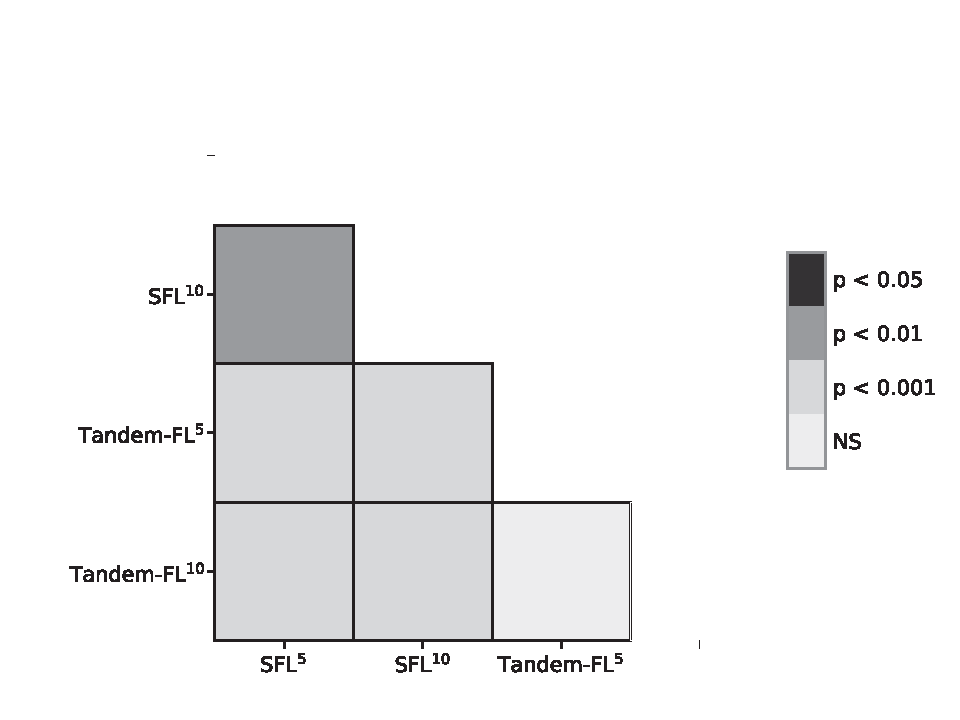
\includegraphics[width=0.45\textwidth]{figures/heatmap_nemenyi_result.pdf}
		\caption{Nemenyi post-hoc analysis results \Sof{Considering \chart{}, \jtime{}, \mockito{}, \lang{} }}
		\label{fig:performance}
\end{figure}

\subsection{Threats to validity}
%
A potential threat to external validity related to the set of programs used in
our study. When choosing the projects for our study, our aim was to opt for
projects that resemble a general and large-sized application. To reduce
selection bias and facilitate the comparison of our results, we decided to
choose a benchmark that is popular in the community \Rui{cite d4j}.

A potential threat to construct validity relates to the choice of oracle generation
for the Lithium toolset. However, we argue that our choice is able to capture whether
a program is failing because of the same reason.

The main threat to internal validity lies in the complexity of several of the tools
used in our experiments, most notably the Lithium toolset, the SFL diagnosis tool,
and the implementation of \comb{}.
%
\section{Related Work}
\Rui{needs work...}

\Mar{moved from intro$\rightarrow$} It is worth noting that Automated
Program Repair techniques should directly benefit from these
results---either to improve their results or to be aware they should
not invest on this integration.

\subsection{Program Slicing}

Program Slicing is an old technique with several applications in PL
and SE research~\cite{Weiser:1981:PS:800078.802557}. Slicing can be
implemented in different ways. Dynamic Slicing has found its main
application in fault
localization~\cite{Agrawal:1990:DPS:93542.93576}---in this application
context, failing tests exist. Research in this area has mainly focused
on slicing code
efficiently~\cite{Wang:2008:DSJ:1330017.1330021,Wang:2004:UCB:998675.999455}
and avoiding data and control omission
errors~\cite{Zhang:2007:TLE:1250734.1250782,Lin:2018:BDE:3238147.3238163}. Omission errors correspond to the
cases where tests fail because some part of the code was not executed
when it should. Dynamic fault localization techniques cannot hope to
soundly report bugs in those cases. The issue is that incorporating
static information to capture those cases can result in unacceptably
large slices, which defeats the purpose of reducing the fault search
space. It is worth noting that, conceptually, the \comb{} combination
can be used with any form of dynamic slicing. We chose an
implementation of Critical
Slicing~\cite{DeMillo:1996:CSS:229000.226310} for its generality.



\subsection{SFL}

Statistics-based techniques (e.g., ~\cite{Pearson:2017:EIF:3097368.3097441}) are
popular automated fault localization techniques within the Software Engineering
community. They correlate information about program fragments that have been
exercised in multiple program execution traces (also called \textit{program
spectra}) with information about successful and failing executions. By doing
that, statistics-based approaches yield a list of suspect program fragments
sorted by their likelihood to be at fault. Since this technique is efficient in
practice, it is attractive for large modern software systems ~\cite{Zoeteweij:2007:DES:1251988.1253298}.

Spectrum-based fault localization (\sfl) is amongst the most common statistical
fault localization technique that takes as input a test suite including at least
one failing test and reports on output a ranked list of components likely to be
in fault ~\cite{FLSurvey2016,DBLP:conf/kbse/JonesH05,DBLP:journals/smr/LuciaLJTB14,DBLP:journals/jss/AbreuZGG09}.

\subsection{\comb{}}
\Rui{\comb{} ??}

Prior work has investigated the combination of dynamic slicing and
spectrum-based fault
localization ~\cite{Wotawa:2010:FLB:1848650.1849235,Alves:2011:FUD:2190078.2190115,DBLP:conf/ecai/HoferW12,lei-mao-dai-wang-2012,slicing-sfl-repair}. Although
the methodology used in these papers vary, the overall message is that
the combination is valuable. Note that slicing alone does not provide
the guarantee of improvement to \sfl{} as statements discarded with
slicing could have been ranked lower compared to faulty
statements. This paper differs from prior work in that it uses a much
larger dataset of programs and faults and a more rigorous experimental
methodology.


\section{Conclusions and Future Work}\label{sec:conc}



%\section*{Acknowledgments}
%include only after review.


{
  \small
  \balance
  \bibliographystyle{named}
  \bibliography{paper}
}

% \begin{appendices}
% 	\section{Other data that might be interesting to report}
% 	This section has the only purpose of presenting and discussing other data that
% 	are not intended yet to be used in the paper. If you find something interesting
% 	in this block of information, please report.
%
% 	\begin{table}[h]
% 		\centering
% 		\setlength{\tabcolsep}{4pt}
% 		\begin{tabular}{ccc}
% 			\toprule
% 			$\Delta$$C$             &  \comb{}-5  & \comb{}-10 \\
% 			\midrule
% 			$<0$  & 19.2\% & 15.4\% \\
% 			$=0$  & 23.1\% & 26.9\% \\
% 			$>0$  & 57.7\% & 57.7\% \\
%
% 			\bottomrule
% 		\end{tabular}
% 		\caption {\chart{} - Diagnosis Performance for using \comb{}-5 and \comb{}-10 instead of \sfl{}}
% 		\label{tab:diagchart}
% 	\end{table}
% 	\normalsize
%
% 	\begin{table}[h]
% 		\centering
% 		\setlength{\tabcolsep}{4pt}
% 		\begin{tabular}{ccc}
% 			\toprule
% 			$\Delta$$C$             &  \comb{}-5  & \comb{}-10 \\
% 			\midrule
% 			$<0$  & 40.7\% & 33.3\% \\
% 			$=0$  & 25.9\% & 18.5\% \\
% 			$>0$  & 33.3\% & 48.1\% \\
%
% 			\bottomrule
% 		\end{tabular}
% 		\caption {\jtime{} - Diagnosis Performance for using \comb{}-5 and \comb{}-10 instead of \sfl{}}
% 		\label{tab:diagtime}
% 	\end{table}
% 	\normalsize
%
%
% 	\begin{table}[h]
% 		\centering
% 		\setlength{\tabcolsep}{4pt}
% 		\begin{tabular}{ccc}
% 			\toprule
% 			$\Delta$$C$             &  \comb{}-5  & \comb{}-10 \\
% 			\midrule
% 			$<0$  & 36.8\% & 28.9\% \\
% 			$=0$  & 26.3\% & 28.6\% \\
% 			$>0$  & 36.8\% & 50.0\% \\
%
% 			\bottomrule
% 		\end{tabular}
% 		\caption {\mockito{} - Diagnosis Performance for using \comb{}-5 and \comb{}-10 instead of \sfl{}}
% 		\label{tab:diagmockito}
% 	\end{table}
% 	\normalsize
%
% 	\begin{table*}[h]
% 		\setlength{\tabcolsep}{3pt}
% 		\begin{tabular}{llllllllllllll}
% 			\toprule
% 			   & 1       & 2       & 3       & 4       & 5       & 6       & 7       & 8       & 9       & 10      & 11      & 12      & 13      \\\midrule
% 		top-5  & 81.46\% & 79.06\% & 80.10\% & 0.00\%  & 50.35\% & 86.30\% & 78.71\% & 78.73\% & 44.47\% & 84.29\% & 82.94\% & 38.90\% & 58.46\% \\
% 		top-10 & 16.71\% & 75.96\% & 35.93\% & 12.16\% & 50.35\% & 86.30\% & 81.02\% & 78.73\% & 54.69\% & 84.29\% & 82.94\% & 20.88\% & 61.85\% \\\midrule
% 			   & 14      & 15      & 16      & 17      & 18      & 19      & 20      & 21      & 22      & 23      & 24      & 25      & 26      \\\midrule
% 		top-5  & 66.23\% & 66.00\% & 51.13\% & 49.24\% & 71.76\% & 69.81\% & 82.82\% & 74.84\% & 46.60\% & 22.11\% & 18.39\% & 78.99\% & 0.00\%  \\
% 		top-10 & 67.43\% & 69.98\% & 47.11\% & 55.59\% & 72.84\% & 68.40\% & 68.85\% & 54.43\% & 46.60\% & 37.50\% & 18.39\% & 45.68\% & 0.00\%  \\
% 			\bottomrule
% 		\end{tabular}
% 		\caption {\ds{} reduction performance for each version of the \chart{} project considering only the top-5 and top-10 classes}
% 		\label{table:reduction}
% 	\end{table*}
%
% 	\begin{table*}[h]
% 		\small
% 		\setlength{\tabcolsep}{3pt}
% 		\begin{tabular}{@{}p{1.6cm}p{1cm}p{1.3cm}p{1cm}p{1cm}p{0.8cm}p{1cm}p{1cm}p{1cm}p{1.1cm}p{1cm}p{1cm}p{1.6cm}p{1.3cm}@{}}
% 		\toprule
% 			   & 1    & 2   & 3  & 4   & 5           & 6   & 7  & 8    & 9            & 10     & 11 & 12      & 13   \\ \midrule
% 		SFL    & 36   & 265.56    & 6.5         & 173 & 7.5         & 57  & 72 & 9.5  & 8.5          & 2.5    & 10 & 19.5    & 44.5 \\
% 		\comb{}-5   & 15.5 & 716.5       & 5           & 107 & 7           & 15  & 44 & 8    & 8.5          & 2      & 6  & 2410    & 35.5 \\
% 		$\Delta-5$  & 56.94\% & -169.80\%   & 23.08\%     & 38.15\% & 6.67\%      & 73.68\% & 38.89\% & 15.79\% & 0.00\%      & 20.00\% & 40.00\% & -12258.97\% & 20.22\%   \\
% 		\comb{}-10  & 35.5 & 406.38     & 5           & 114 & 7           & 15  & 46 & 8    & 8.5          & 2      & 6  & 2448    & 35.5 \\
% 		$\Delta-10$ & 1.39\%  & -53.02\%    & 23.08\%     & 34.10\% & 6.67\%      & 73.68\% & 36.11\% & 15.79\% & 0.00\%      & 20.00\% & 40.00\% & -12453.85\% & 20.22\%   \\\midrule
% 		& 14   & 15          & 16          & 17  & 18          & 19  & 20 & 21   & 22           & 23     & 24 & 25      & 26   \\\midrule
% 		SFL    & 15.5 & 2471.17 & 13.5        & 2   & 9.5         & 3.5 & 6  & 39   & 57.21  & 6818.5 & 3  & 3516    & 140  \\
% 		\comb{}-5   & 15.5 & 2254.17 & 9.17 & 2   & 7.67 & 2.5 & 6  & 21   & 105.43  & 6818.5 & 3  & 6046.5  & 717  \\
% 		$\Delta-5$  & 0.00\%  & 8.78\%      & 32.10\%     & 0.00\%  & 19.30\%     & 28.57\% & 0.00\%  & 46.15\% & -84.27\%    & 0.00\%  & 0.00\%  & -71.97\%    & -412.14\% \\
% 		\comb{}-10  & 15.5 & 2264.83 & 10.83 & 2   & 7.67 & 2.5 & 6  & 29.5 & 105.43  & 6818.5 & 3  & 6063.5  & 140  \\
% 		$\Delta-10$ & 0.00\%  & 8.35\%      & 19.75\%     & 0.00\%  & 19.30\%     & 28.57\% & 0.00\%  & 24.36\% & -84.27\%    & 0.00\%  & 0.00\%  & -72.45\%    & 0.00\% \\
% 		\bottomrule
% 		\end{tabular}
% 		\caption {Reporting the rank of all faulty statements obtained by appling \sfl{}, \comb{}-5 and \comb{}-10 to each version of the \chart{} project and performance evaluation of applying \ds{} to \sfl{} considering the top-5 ($\Delta-5$) and top-10 ($\Delta-10$) of the faulty classes}
% 		\label{table:performance}
% 	\end{table*}
% 	\normalsize


% \end{appendices}

\end{document}
